%! TEX root = ../BimodalReference.tex
\documentclass[../BimodalReference.tex]{subfiles}
\begin{document}

\section{Metalogic}

The metalogic for the bimodal logic \textbf{TM} establishes that the proof system and semantics describe the same space of inferences.
This chapter presents a representation theorem from which completeness and compactness follow as corollaries.
The chapter also proves that \textbf{TM} is decidable.

\subsection{Soundness}

This theorem establishes that only logical consequences are derivable.

\begin{theorem}[Soundness]
If $\context \proves \varphi$ then $\context \satisfies \varphi$.
\end{theorem}

The proof proceeds by induction on the derivation structure:
\begin{itemize}
  \item \textbf{Axioms}: Each of the 14 axiom schemata is proven valid
  \item \textbf{Assumptions}: Assumed formulas are true by hypothesis
  \item \textbf{Modus ponens}: Validity preserved under implication elimination
  \item \textbf{Necessitation}: Valid formulas become necessarily valid
  \item \textbf{Temporal necessitation}: Valid formulas become always-future valid
  \item \textbf{Temporal duality}: Past-future swap preserves validity
  \item \textbf{Weakening}: Adding premises preserves semantic consequence
\end{itemize}

\begin{center}
\begin{tabular}{@{}lll@{}}
\toprule
Axiom Validity & Lean Theorem & Technique \\
\midrule
\texttt{prop\_k\_valid} & Propositional K & Propositional reasoning \\
\texttt{prop\_s\_valid} & Propositional S & Propositional reasoning \\
\texttt{ex\_falso\_valid} & EFQ & Vacuous implication \\
\texttt{peirce\_valid} & Peirce & Classical case analysis \\
\texttt{modal\_t\_valid} & MT & Reflexivity of accessibility \\
\texttt{modal\_4\_valid} & M4 & Transitivity of accessibility \\
\texttt{modal\_b\_valid} & MB & Symmetry of accessibility \\
\texttt{modal\_5\_collapse\_valid} & M5 & S5 equivalence structure \\
\texttt{modal\_k\_dist\_valid} & MK & Distribution \\
\texttt{temp\_k\_dist\_valid} & TK & Temporal distribution \\
\texttt{temp\_4\_valid} & T4 & Transitivity of time \\
\texttt{temp\_a\_valid} & TA & Temporal connectedness \\
\texttt{temp\_l\_valid} & TL & Always implies recurrence \\
\texttt{modal\_future\_valid} & MF & Time-shift invariance \\
\texttt{temp\_future\_valid} & TF & Time-shift invariance \\
\bottomrule
\end{tabular}
\end{center}

\noindent
The MF and TF axioms use time-shift invariance to relate truth at different times (via \texttt{WorldHistory.time\_shift}).

\subsection{Core Infrastructure}

The completeness proof requires three foundational components including the deduction theorem, maximal consistent sets, and Lindenbaum's lemma.
These provide the infrastructure for constructing canonical models.

\subsubsection{Deduction Theorem}

\begin{theorem}[Deduction Theorem]
If $A :: \context \proves B$ then $\context \proves A \imp B$.
\end{theorem}

The proof uses well-founded induction on derivation height, handling each of the following rules:
\begin{itemize}
  \item \textbf{Axiom}: Use S axiom to weaken
  \item \textbf{Assumption}: Identity if same, S axiom if different
  \item \textbf{Modus ponens}: Use K axiom distribution
  \item \textbf{Weakening}: Case analysis on assumption membership
  \item \textbf{Modal/temporal rules}: Do not apply (require empty context)
\end{itemize}


\subsubsection{Consistency}

\begin{definition}[Consistent]
A context $\context$ is \textbf{consistent} if $\context \not\proves \falsum$.
\end{definition}

\begin{definition}[Maximal Consistent]
A context $\context$ is \textbf{maximal consistent} if it is consistent and
for all $\varphi \notin \context$, the context $\varphi :: \context$ is inconsistent.
\end{definition}

\begin{definition}[Negation-Complete]
A set of formulas $S$ is \textbf{negation-complete} if for every formula $\varphi$, exactly one of $\varphi$ or $\lneg\varphi$ is in $S$.
\end{definition}

Maximal consistent sets (MCS) are negation-complete.
This property is essential for defining canonical world states, as it ensures that every formula has a definite truth value in each MCS.

\subsubsection{Lindenbaum's Lemma}

\begin{lemma}[\texttt{set\_lindenbaum}]
Every consistent context can be extended to a maximal consistent context.
\end{lemma}

The proof applies Zorn's lemma to the partially ordered set of consistent supersets of the given context.
Note that contexts (finite lists of formulas) embed naturally into sets, so ``consistent context'' and ``consistent set'' are used interchangeably here.
The key step is showing that the union of any chain of consistent sets is itself consistent.
This follows because any derivation uses only finitely many premises, so a derivation of $\falsum$ from the union would have to come from some finite subset, which is contained in some member of the chain, contradicting that member's consistency.

\subsection{Representation Theory}

The \emph{Representation Theorem} is the core of the metalogic, providing the bridge between syntactic consistency and semantic satisfiability.
The subsequent \emph{Completeness Theorems} follow directly from this result.

\subsubsection{Canonical World States}

The semantic approach constructs world states from histories and times.
We first define these constituent concepts before assembling them into canonical structures.

% FIX: these definitions are not accurate or formally precise

\begin{definition}[History]
A \textbf{history} is a function $\tau : \mathbb{Z} \to \text{MCS}$ mapping each time to a maximal consistent set, satisfying temporal coherence: for each time $t$, the formulas in $\tau(t)$ are consistent with the temporal operators applied to formulas in $\tau(t')$ for related times $t'$.
\end{definition}

\begin{definition}[Time]
\textbf{Times} are integers ($\mathbb{Z}$), providing a discrete linear order with both past and future directions.
\end{definition}

\begin{definition}[Task Relation]
The \textbf{task relation} (\texttt{SemanticTaskRelV2}) relates world states based on the existence of histories connecting them: world state $w$ is task-related to $w'$ if there exists a history $\tau$ such that $w$ and $w'$ both occur along $\tau$.
\end{definition}

% TODO: I don't see how the integers can be used without making time discrete. Rather, a canonical frame should have the same structural properties as the definition of a frame in the semantics where a temporal order is ANY totally ordered commutative group. This is the crux of the proof strategy and so needs careful thinking and research.

% FIX: this should be moved into the definition below, calling this the 'canonical world state', not 'semantic world state'

A \textbf{canonical world state} is derived from a maximal consistent set.
The semantic approach defines world states as equivalence classes of (history, time) pairs.

\begin{definition}[Semantic World State]
A world state is an equivalence class of (history, time) pairs under the relation where two pairs are equivalent iff they denote the same underlying world state.\footnote{This is formalized as \texttt{SemanticWorldState}.}
\end{definition}

% TODO: it would be nice if SemanticCanonicalFrame in the lean source code was renamed CanonicalTaskFrame since this is more accurate

\begin{definition}[\texttt{SemanticCanonicalFrame}]
The \textbf{canonical semantic frame} has:
\begin{itemize}
  \item World states: Equivalence classes of history-time pairs over maximal consistent sets
  \item Times: Integers ($\mathbb{Z}$)
  \item Task relation: Defined via history existence (\texttt{SemanticTaskRelV2})
\end{itemize}
The frame satisfies nullity and compositionality.
\end{definition}

\begin{definition}[Canonical Valuation]
An atom $p$ is true at world state $[\tau, x]$ iff $p \in \mathsf{MCS}(\tau(x))$.
\end{definition}

\begin{lemma}[Truth Lemma]
In the semantic canonical model, $\varphi \in \mathsf{MCS}(\tau(x))$ iff $\varphi$ is true at world state $[\tau, x]$.\footnote{This is proven as \texttt{semantic\_truth\_lemma\_v2}.}
\end{lemma}

% TODO: This is not in the correct spirit of a representation theorem which aims to build a semantic object out of pure syntax. A purely syntactic, and fully general approach should be carefully researched and implemented, thinking hardest about this crux of the metalogic.

The \emph{quotient construction} identifies (history, time) pairs that agree on which formulas hold, forming equivalence classes.
Two pairs $(\tau_1, t_1)$ and $(\tau_2, t_2)$ are equivalent when $\tau_1(t_1) = \tau_2(t_2)$ as maximal consistent sets.
The \emph{Truth Lemma} follows directly from this construction: membership in a maximal consistent set corresponds to truth by definition of the equivalence class.

\subsubsection{Representation Theorem}

\begin{theorem}[Representation Theorem (\texttt{representation\_theorem})]
Every consistent context is satisfiable in the canonical model.
\end{theorem}

This theorem is the pivotal result linking syntax to semantics.
The proof strategy is:
\begin{enumerate}
  \item Given a consistent context $\context$, convert it to a set $S = \texttt{contextToSet}(\context)$.
  \item Apply Lindenbaum's lemma to extend $S$ to a maximal consistent set $M$.
  \item View $M$ as a canonical world state.
  \item By the truth lemma, all formulas in $\context$ are satisfied at this world.
\end{enumerate}

The elegance of this approach is that the MCS construction makes the \emph{Truth Lemma} essentially trivial since truth \emph{is} membership in the MCS.

\begin{theorem}[Strong Representation Theorem]
If $\context \not\proves \varphi$, then $\context \cup \{\lneg\varphi\}$ is satisfiable in the canonical model.\footnote{This is proven as \texttt{strong\_representation\_theorem}.}
\end{theorem}

This strengthening is crucial for completeness: it says that any formula unprovable from a context can be made false while satisfying the context.
The proof adds $\lneg\varphi$ to the context and applies the standard \emph{Representation Theorem} to the resulting consistent set.

\subsubsection{Theorem Dependency Structure}

\Cref{fig:theorem-deps} illustrates the dependency structure of the completeness proof.
The core infrastructure (top row) feeds into the central \emph{Representation Theorem}, from which the completeness corollaries follow.

\begin{figure}[ht]
\centering
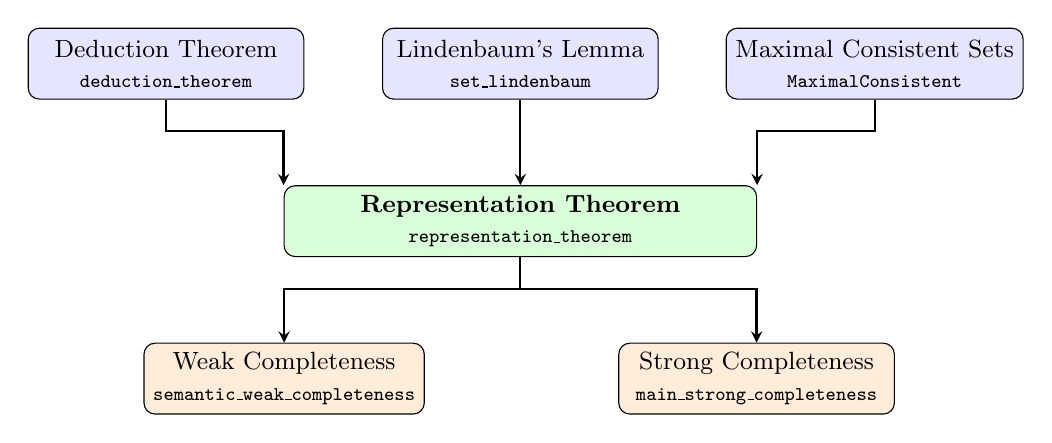
\begin{tikzpicture}[
  box/.style={rectangle, draw, rounded corners, minimum width=3.5cm, minimum height=0.9cm, align=center, font=\small},
  arrow/.style={->, >=stealth, thick}
]
  % Core Infrastructure layer (top)
  \node[box, fill=blue!10] (deduct) at (0,4) {Deduction Theorem\\{\scriptsize\texttt{deduction\_theorem}}};
  \node[box, fill=blue!10] (linden) at (4.5,4) {Lindenbaum's Lemma\\{\scriptsize\texttt{set\_lindenbaum}}};
  \node[box, fill=blue!10] (mcs) at (9,4) {Maximal Consistent Sets\\{\scriptsize\texttt{MaximalConsistent}}};

  % Representation layer (middle) - central
  \node[box, fill=green!15, minimum width=6cm] (repr) at (4.5,2) {\textbf{Representation Theorem}\\{\scriptsize\texttt{representation\_theorem}}};

  % Completeness layer (bottom)
  \node[box, fill=orange!15] (weak) at (1.5,0) {Weak Completeness\\{\scriptsize\texttt{semantic\_weak\_completeness}}};
  \node[box, fill=orange!15] (strong) at (7.5,0) {Strong Completeness\\{\scriptsize\texttt{main\_strong\_completeness}}};

  % Arrows from Core to Representation
  \draw[arrow] (deduct.south) -- ++(0,-0.4) -| (repr.north west);
  \draw[arrow] (linden.south) -- (repr.north);
  \draw[arrow] (mcs.south) -- ++(0,-0.4) -| (repr.north east);

  % Arrows from Representation to Completeness
  \draw[arrow] (repr.south) -- ++(0,-0.4) -| (weak.north);
  \draw[arrow] (repr.south) -- ++(0,-0.4) -| (strong.north);
\end{tikzpicture}
\caption{Theorem dependency structure for completeness.}
\label{fig:theorem-deps}
\end{figure}

The three foundational components---the \emph{Deduction Theorem}, \emph{Lindenbaum's Lemma}, and \emph{Maximal Consistent Sets}---provide the infrastructure for the \emph{Representation Theorem}.
Both weak and strong completeness then follow as direct corollaries via contrapositive arguments.

\subsection{Completeness as Corollary}

The \emph{Completeness Theorems} follow directly from the \emph{Representation Theorem} via contrapositive arguments.

\subsubsection{Weak Completeness}

\begin{theorem}[Weak Completeness]
If $~\satisfies{\varphi}$, then $\proves \varphi$.\footnote{This is proven as \texttt{semantic\_weak\_completeness}.}
\end{theorem}

The proof proceeds by contraposition:
\begin{enumerate}
  \item Assume $\not\proves \varphi$ (i.e., the empty context does not derive $\varphi$).
  \item Then $\{\lneg\varphi\}$ is consistent (otherwise we could derive $\varphi$).
  \item By the \emph{Representation Theorem}, $\{\lneg\varphi\}$ is satisfiable in the canonical model.
  \item So there exists a world where $\lneg\varphi$ is true, meaning $\varphi$ is false.
  \item Hence $\varphi$ is not valid.
\end{enumerate}
By contraposition, validity implies provability.

\subsubsection{Strong Completeness}

% TODO: This still leaves infinite contexts/sets remaining to be addressed, where this should be addressed by compactness

\begin{theorem}[Strong Completeness]
If $\context \satisfies \varphi$, then $\context \proves \varphi$.\footnote{This is proven as \texttt{main\_strong\_completeness} with bridge sorries for the generalization.}
\end{theorem}

The proof extends weak completeness using an implication chain technique:
\begin{enumerate}
  \item Assume semantic consequence: $\context \satisfies \varphi$.
  \item For context $\context = [\psi_1, \ldots, \psi_n]$, build the implication chain $\psi_1 \imp (\psi_2 \imp \cdots (\psi_n \imp \varphi))$.
  \item Show this chain is valid (from the semantic consequence assumption).
  \item By weak completeness, the chain is provable.
  \item Unfold the chain with repeated modus ponens applications to obtain $\context \proves \varphi$.
\end{enumerate}

% TODO: it would be better to state this in the strong formulation with contexts behind each turnstile. Both in the latex and lean code, the strong formulations should be the real focus, introducing the weak formulations only where it is useful.

\begin{theorem}[Provable iff Valid]
$\proves \varphi \iff \satisfies{\varphi}$.\footnote{This is proven as \texttt{main\_provable\_iff\_valid}, establishing completeness of \textbf{TM}.}
\end{theorem}

This biconditional shows that the proof system and semantics align perfectly.
Soundness (left-to-right) ensures no non-logical consequences are derivable, while completeness (right-to-left) ensures all logical consequences are captured by the proof system.
Together, they establish that \textbf{TM} provides an exact syntactic characterization of semantic validity.

\subsubsection{Two Canonical Model Approaches}

The codebase contains two canonical model constructions.
Understanding their differences explains why the semantic approach is primary.

% TODO: the following syntactic approach is in the correct spirit and should be ported over from the Boneyard. This is deserving of careful study to implement completely. By contrast, the semantic approach abandons the intended spirit of the representation theorem.

\paragraph{Syntactic Approach.}
World states are directly identified with maximal consistent sets.
Accessibility is defined via modal witnesses: $\nec\varphi \in w$ implies $\varphi \in w'$ for all accessible $w'$.
This approach requires explicit negation-completeness proofs for locally consistent sets.
The syntactic approach is archived in \texttt{Boneyard/} for historical reference.

\paragraph{Semantic Approach.}
World states are equivalence classes of (history, time) pairs, where two pairs are equivalent iff they denote the same underlying world state.
This approach offers key advantages:
\begin{itemize}
  \item \textbf{Truth lemma}: Follows trivially from the quotient construction.
  \item \textbf{Compositionality}: The task relation is defined via history concatenation, making compositionality proofs straightforward.
  \item \textbf{Negation-completeness}: The semantic approach does not require proving negation-completeness of arbitrary locally consistent sets, a property that caused difficulties in the syntactic approach.
\end{itemize}

\subsection{Decidability}

The decidability of TM bimodal logic rests on the \emph{Finite Model Property}: if a formula is satisfiable, it is satisfiable in a finite model bounded by the formula's modal and temporal depth.
The bound on model size is $2^{|\mathsf{closure}(\varphi)|}$, where the subformula closure contains all relevant formulas for determining the truth of $\varphi$.
This property connects the representation infrastructure to decidability by ensuring that satisfiability checking can terminate.

The decidability proof proceeds via a tableau-based decision procedure.

\begin{theorem}[Decidability]
Validity in TM bimodal logic is decidable: for any formula $\varphi$, either $\valid{\varphi}$ or $\neg\valid{\varphi}$.
\end{theorem}

\begin{theorem}[Decision Soundness]
If the decision procedure returns ``valid'' with proof $\pi$, then $\valid{\varphi}$.\footnote{This is proven as \texttt{decide\_sound}.}
\end{theorem}

Here $\pi$ is a derivation term witnessing $\proves \varphi$, constructed from the closed tableau.
In Lean 4, this is a term of type \texttt{ContextDerivable [] $\varphi$}, representing a formal proof tree.

The decision procedure operates as follows:
\begin{enumerate}
  \item \textbf{Direct axiom proof}: Check if $\varphi$ matches one of the axiom schemata directly, yielding an immediate derivation.
  \item \textbf{Proof search}: Apply Lean 4 tactics (\texttt{decide}, \texttt{simp}) with bounded recursion depth to find a derivation automatically.
  \item \textbf{Tableau construction}: Build a systematic tree that decomposes $\varphi$ into simpler signed formulas.
  \item If all branches close: formula is valid, extract proof.
  \item If open saturated branch: formula is invalid, extract countermodel.
\end{enumerate}

A \emph{tableau} is a tree-structured refutation method: to prove $\varphi$ valid, we assume $\varphi$ is false and systematically derive contradictions.
Each branch represents a possible scenario; if all branches lead to contradictions, the original assumption was impossible, so $\varphi$ must be valid.

\subsubsection{Tableau Structure}

The tableau uses \textbf{signed formulas} with annotations:
\begin{itemize}
  \item $T(\varphi)$: formula $\varphi$ is assumed true
  \item $F(\varphi)$: formula $\varphi$ is assumed false
\end{itemize}

\textbf{Expansion rules} are categorized as:
\begin{itemize}
  \item \textbf{Propositional}: $T(\varphi \land \psi)$ splits, $F(\varphi \imp \psi)$ splits, etc.
  \item \textbf{Modal}: $T(\nec\varphi)$ propagates to accessible worlds, $F(\poss\varphi)$ creates witness
  \item \textbf{Temporal}: $T(\always\varphi)$ propagates to future times, $F(\sometimes\varphi)$ creates witness
\end{itemize}

\noindent
A branch \textbf{closes} when it contains both $T(\varphi)$ and $F(\varphi)$ for some formula.
A branch is \textbf{saturated} when no expansion rules apply.

\subsubsection{Complexity}

\begin{center}
\begin{tabular}{@{}ll@{}}
\toprule
Measure & Complexity \\
\midrule
Time & $O(2^n)$ where $n$ is formula size \\
Space & $O(n)$ \\
Class & PSPACE-complete \\
\bottomrule
\end{tabular}
\end{center}

The exponential time bound means formulas of modest size (30--50 symbols) remain tractable on modern hardware.
PSPACE-completeness implies that modal satisfiability is among the hardest problems solvable with polynomial space, but the linear space bound makes memory usage manageable even for larger formulas.

% TODO: it would also help to explain where the calculations come from (how these numbers are calculated) and check that they are in fact correct as stated

\subsubsection{Decision Result Types}

The decision procedure returns one of three outcomes:
\begin{itemize}
  \item \texttt{valid proof}: Formula is valid with derivation tree
  \item \texttt{invalid counter}: Formula is invalid with countermodel
  \item \texttt{timeout}: Resources exhausted before decision
\end{itemize}

Despite computational limitations, decidability is practically valuable: small formulas (most proof obligations in practice) resolve quickly, invalid formulas are often rejected early without full exploration, and countermodels provide concrete feedback for debugging specifications.

\subsection{File Organization and Dependencies}

The \texttt{Metalogic\_v2} directory contains 27 Lean files organized into six subdirectories.
The following diagram illustrates the import structure, showing how files depend on each other.

\begin{center}
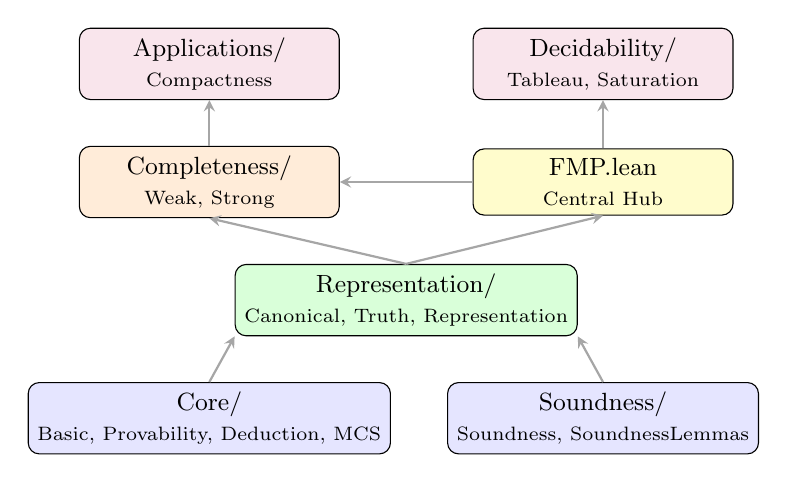
\begin{tikzpicture}[
  dirbox/.style={rectangle, draw, rounded corners, minimum width=3.3cm, minimum height=0.7cm, align=center, font=\small},
  arrow/.style={->, >=stealth, thick, gray!70}
]
  % Core layer (bottom)
  \node[dirbox, fill=blue!10] (core) at (0,0) {Core/\\{\scriptsize Basic, Provability, Deduction, MCS}};
  \node[dirbox, fill=blue!10] (sound) at (5,0) {Soundness/\\{\scriptsize Soundness, SoundnessLemmas}};

  % Representation layer (middle)
  \node[dirbox, fill=green!15] (repr) at (2.5,1.5) {Representation/\\{\scriptsize Canonical, Truth, Representation}};

  % Completeness layer
  \node[dirbox, fill=orange!15] (compl) at (0,3) {Completeness/\\{\scriptsize Weak, Strong}};

  % FMP hub
  \node[dirbox, fill=yellow!20] (fmp) at (5,3) {FMP.lean\\{\scriptsize Central Hub}};

  % Applications and Decidability
  \node[dirbox, fill=purple!10] (apps) at (0,4.5) {Applications/\\{\scriptsize Compactness}};
  \node[dirbox, fill=purple!10] (decid) at (5,4.5) {Decidability/\\{\scriptsize Tableau, Saturation}};

  % Arrows
  \draw[arrow] (core.north) -- (repr.south west);
  \draw[arrow] (sound.north) -- (repr.south east);
  \draw[arrow] (repr.north) -- (compl.south);
  \draw[arrow] (repr.north) -- (fmp.south);
  \draw[arrow] (compl.north) -- (apps.south);
  \draw[arrow] (fmp.north) -- (decid.south);
  \draw[arrow] (fmp.west) -- (compl.east);
\end{tikzpicture}
\end{center}

\noindent
\textbf{Directory descriptions}:
\begin{itemize}
  \item \textbf{\texttt{Core/}}: Foundational definitions including provability (\texttt{ContextDerivable}), deduction theorem, and maximal consistent sets.
  \item \textbf{\texttt{Soundness/}}: Validity proofs for all 15 axiom schemata and the main soundness theorem.
  \item \textbf{\texttt{Representation/}}: Canonical model construction, truth lemma, and the central representation theorems.
  \item \textbf{\texttt{Completeness/}}: Weak and strong completeness theorems derived from representation.
  \item \textbf{\texttt{Applications/}}: Compactness theorem (trivial for list-based contexts).
  \item \textbf{\texttt{Decidability/}}: Tableau-based decision procedure with proof/countermodel extraction.
\end{itemize}

\subsection{Implementation Status}

\subsubsection{Sorry Status}

The \texttt{Metalogic\_v2} codebase has three remaining \texttt{sorry} statements, none of which block the core completeness results:

\begin{enumerate}
  \item \texttt{semantic\_task\_rel\_compositionality} (SemanticCanonicalModel.lean:236) --- Finite time domain limitation; a fundamental issue with Int-valued durations exceeding finite time bounds.
  \item \texttt{main\_provable\_iff\_valid\_v2} completeness direction (SemanticCanonicalModel.lean:647) --- Requires truth bridge from general validity to finite model truth.
  \item \texttt{finite\_model\_property\_constructive} truth bridge (FiniteModelProperty.lean:481) --- Same truth bridge issue.
\end{enumerate}

\noindent
The core completeness result \texttt{semantic\_weak\_completeness} is fully proven without sorries.

\subsubsection{Decidability Implementation}

\begin{center}
\begin{tabular}{@{}lll@{}}
\toprule
Submodule & Status & Notes \\
\midrule
SignedFormula & Complete & Sign, SignedFormula, Branch types \\
Tableau & Complete & Expansion rules \\
Closure & Complete & Branch closure detection \\
Saturation & Complete & Fuel-based termination \\
ProofExtraction & Partial & Axiom instances only \\
CountermodelExtraction & Complete & From open branches \\
DecisionProcedure & Complete & Main decide function \\
Soundness & Proven & \texttt{decide\_sound} \\
Completeness & Partial & Requires Finite Model Property \\
\bottomrule
\end{tabular}
\end{center}

\subsubsection{Metalogic Implementation}

\begin{center}
\begin{tabular}{@{}lll@{}}
\toprule
Component & Status & Lean \\
\midrule
Soundness & Proven & \texttt{soundness} \\
Deduction Theorem & Proven & \texttt{deduction\_theorem} \\
Lindenbaum Lemma & Proven & \texttt{set\_lindenbaum} \\
Canonical Frame & Proven & \texttt{SemanticCanonicalFrame} \\
Truth Lemma & Proven & \texttt{semantic\_truth\_lemma\_v2} \\
Representation Theorem & Proven & \texttt{representation\_theorem} \\
Weak Completeness & Proven & \texttt{semantic\_weak\_completeness} \\
Strong Completeness & Proven* & \texttt{main\_strong\_completeness} \\
Provable iff Valid & Proven & \texttt{main\_provable\_iff\_valid} \\
Finite Model Property & Statement & \texttt{finite\_model\_property} \\
Decidability Soundness & Proven & \texttt{decide\_sound} \\
\bottomrule
\end{tabular}
\end{center}

\noindent
* Strong completeness uses the weak completeness result, which is fully proven.
The three sorries listed above affect only the finite model property path.

\end{document}
